\documentclass[a4,10pt,oneside,openany]{ctexart}
\usepackage[utf8x]{inputenc}
%\usepackage[UTF8]{ctex}
%\usepackage[english]{babel}
\usepackage{mathpazo}
\usepackage{mathrsfs}
\setlength{\parskip}{0.2\baselineskip}
%\setlength{\parskip}{0.2em}
\usepackage{url}
\usepackage{amssymb,amsmath,amsthm,amsfonts}
\usepackage{mathtools}
\usepackage{geometry}
\usepackage{float}
\usepackage{tikz}
\tikzset{elegant/.style={smooth,thick,samples=50,cyan}}
\tikzset{eaxis/.style={->,>=stealth}}


\usepackage{extarrows}
\usepackage{subfigure}
\usepackage{graphics}
\usepackage{wrapfig}
\usepackage{graphicx}
\usepackage{enumerate}
\usepackage{subfigure}
\usepackage{CJKulem}%中文删除线
\usepackage[normalem]{ulem} % \sout{想加删除线的中文}
\usepackage{picinpar}%图片绕排,是真滴烦
\usepackage{float}

%页眉页脚
\usepackage{authblk}
\usepackage{fancyhdr}
\usepackage{lastpage}

%以下是书写伪代码用
\usepackage{algorithm}  
\usepackage{algpseudocode}  
\renewcommand{\algorithmicrequire}{\textbf{Input:}}  % Use Input in the format of Algorithm  
\renewcommand{\algorithmicensure}{\textbf{Output:}} % Use Output in the format of Algorithm 

\geometry{a4paper, left=3cm, right=3cm, bottom=3cm, top=3cm}%此行定义了纸张大小和边距,不需要可删除

%以下是Inkspace
\usepackage{import}
\usepackage{xifthen}
\usepackage{pdfpages}
\usepackage{transparent}

\usepackage{verbatim}%comment 环境
%\usepackage[backref]{hyperref} %参考文献高亮跳转\\
\usepackage[colorlinks, linkcolor=black, anchorcolor=blue, citecolor=red]{hyperref}

\newcommand{\incfig}[1]{%
\def\svgwidth{\columnwidth}
\import{./figures/}{#1.pdf_tex}
}

\newtheorem{deff}{定义}[section]
\newtheorem{thm}{定理}[section]
\newtheorem{clm}[thm]{命题}
\newtheorem{lemma}[thm]{引理}
\newtheorem{prf}{证明}[section]


\renewcommand{\proofname}{\indent Pr}
\renewcommand{\qedsymbol}{$\blacksquare$}    % 证毕符号改成黑色的正方形

\newcommand{\argmin}[1]{\underset{#1}{\arg \min}\ }
\newcommand{\ceil}[1]{\left\lceil #1 \right \rceil }
\newcommand{\norm}[1]{\left \Vert #1 \right \Vert}
\newcommand{\tform}[1]{\left \Vert #1 \right \Vert_2}
\newcommand{\tnorm}[1]{\left \Vert #1 \right \Vert_2}
\newcommand{\onorm}[1]{\left \Vert #1 \right \Vert_1}
\newcommand{\abs}[1]{\left|#1 \right|}
\newcommand{\var}[1]{\text{Var}\left[ #1\right]}
\newcommand{\xk}[1]{\left( #1\right)} 
\newcommand{\zk}[1]{\left[ #1\right]} 
\newcommand{\dk}[1]{\left\{ #1\right\}} 
\newcommand{\bd}[1]{\bold{#1}}

%量子力学符号------
\newcommand{\xde}{\text{Schrödinger}}
\newcommand{\avg}[1]{\left \langle #1 \right \rangle}
\newcommand{\lvec}[1]{\left \langle #1 \right |}
\newcommand{\rvec}[1]{\left | #1 \right \rangle}


\newtheorem{lproof}{证明}[section]
\newtheorem{tuilun}{推论}
\newtheorem{eg}{例}[section]
\newtheorem{solve}{解}[section]
\newcommand\ii{\textup{i}}
\newcommand\dd{\mathrm{d}}


%自定义数学符号
\newcommand{\diag}{\textup{diag}}
\newcommand{\Frobenius}[1]{\left\Vert #1 \right\Vert}
\newcommand{\fform}[1]{\left\Vert #1 \right\Vert_F}
\newcommand{\parr}[2]{\frac{\partial #1}{\partial #2}}%一阶偏微分
\newcommand{\parrr}[2]{\frac{\partial^2 #1}{\partial #2^2}}%二阶偏微分
\newcommand{\lap}[1]{\parrr{#1}{x} + \parrr{#1}{y} = 0}%二元拉普拉斯方程
\newcommand{\ddd}[2]{\frac{\textup{d} #1}{\textup{d} #2}}%微商
\newcommand{\dddd}[2]{\frac{\textup{d}^2 #1}{\textup{d} #2^2}}%微商

%二重以上环路积分,强迫症了属于是
\def\ooint{{\bigcirc}\kern-11.5pt{\int}\kern-6.5pt{\int}}
\def\oooint{{\bigcirc}\kern-12.3pt{\int}\kern-7pt{\int}\kern-7pt{\int}}


\newcommand{\tu}{\textup}
\newcommand{\bm}{\boldsymbol}
\newcommand{\ol}[1]{$\overline{#1}$}
\newcommand{\re}[1]{\textup{Re}(#1)}
\newcommand{\im}[1]{\textup{Im}(#1)}
\newcommand{\fa}{\forall}
\newcommand{\ex}{\exists}
\newcommand{\st}{\textup{  s.t. }}
\newcommand{\ve}{\varepsilon}
\newcommand{\disp}{\displaystyle}
\newcommand{\chj}{\textup{Cauchy}积分公式}
\newcommand{\res}[1]{\textup{Res}\left(#1\right)}
\newcommand{\mysum}[1][n]{\sum_{i = 1}^{#1}}%求和
\newcommand{\series}[1]{\sum_{n = 0}^{\infty} #1_{n}}%级数
\newcommand{\seriesa}[1]{\sum_{n = 0}^{\infty} \left| #1_{n}\right|}%绝对级数
\newcommand{\fseries}[1]{\sum_{k = 1}^{\infty} #1_k (z)}

\newcommand*{\num}{pi}

%书写横线
\newcommand{\horrule}[1]{\rule[0.5ex]{\linewidth}{#1}} 	% Horizontal rule

% 文档标题
\title{
{\normalfont\normalsize\textsc{
Peking University\\
Introduction to Computer Vision, Spring 2024 \\[25pt]}}
\horrule{0.5pt}\\
\sffamily{Introduction to Computer Vision\\Course Notes}\\
\horrule{1.8pt}\\[20pt]
}

% 作者和联系方式
\author[1]{Prof. He Wang\thanks{\href{https://hughw19.github.io/}{Prof. He Wang}}}
\author[2]{林晓疏\thanks{wangyuanqing@pku.edu.cn}}
\author[2]{Yutong Liang\thanks{\href{https://lyt0112.com/}{Yutong Liang's Website}}}
\affil[1]{主讲教师}
\affil[2]{笔记整理}

% 文档日期
\date{\today}

\pagestyle{fancy}
\fancyhf{}
\fancyhead[L]{\leftmark}  % 在页眉左侧显示章节名
\fancyfoot[C]{\thepage}  % 在页脚中间显示页码

\begin{document}


\section{Edge Detection}
 
\subsection{What is an Edge?}

“边缘”是图像中的一个区域,在这个区域中,沿着图像的一个方向,
像素强度值 (或者说对比度) 发生了“显著”的变化,而在其正交方向上,
像素强度值 (或对比度) 几乎没有变化.

\subsection{Criteria for Optimal Edge Detection}

\begin{equation}
\text{Accuracy}=\frac{\text{TP}+\text{TN}}{\text{TP}+\text{FP}+\text{TN}+\text{FN}} 
\end{equation}

\begin{equation}
\text{Precision}=\frac{\text{TP}}{\text{TP}+\text{FP}} 
\end{equation}

\begin{equation}
\text{Recall}=\frac{\text{TP}}{\text{TP}+\text{FN}}
\end{equation}

Precision 和 Recall 都代表着你检测出的真正边缘所占比例,但是 Precision 的分母
是你检测出的边缘,Recall 的分母是真正的边缘.

\subsection{Non-Maximal Suppression (NMS)}

非最大值抑制,顾名思义,就是抑制非最大值,这里的最大值指的是梯度的局部最大值.

在计算出了所有点的梯度之后,会有很多像素的梯度大于设定的阈值,而我们希望最后得出的边缘像素真的看起来
像一条线而不是一块区域,所以 NMS 的目的是为了抑制那些不是边缘的像素,只保留那些是边缘的像素.

\begin{figure}[htbp]
    \centering
	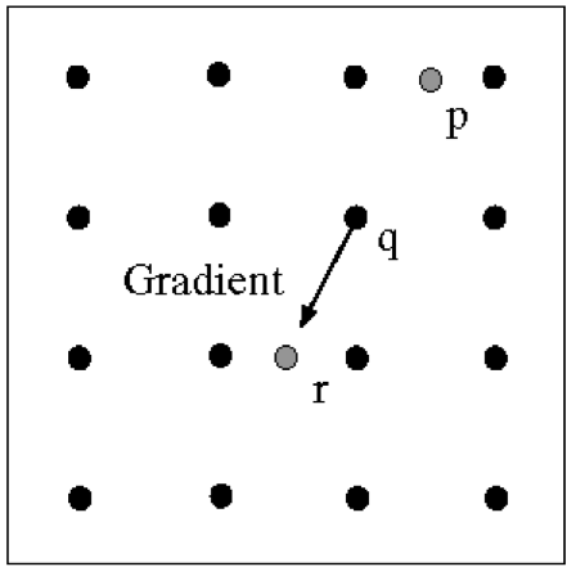
\includegraphics[scale=0.2]{figures/NMS.png}
	\caption{NMS示意图}
\end{figure}

对于一个边缘像素的候选点,我们认为它是边缘当:它比它梯度方向的两个点 $q+\nabla q$ 和 $q-\nabla q$ 的梯度值大,
也就是这个点的梯度大小是局部最大值的时候.

\begin{figure}[htbp]
    \centering
	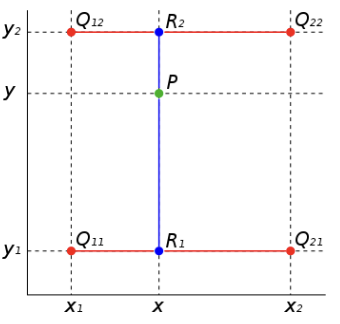
\includegraphics[scale=0.4]{figures/bilinear.png}
	\caption{双线性插值}
\end{figure}

计算这个点梯度方向的点的梯度值可以使用双线性插值法,就是把这个点周围的四个点的梯度按照横纵距离反比加权.

当然,NMS 是一个思想而不是针对边缘检测的算法,比如对于 keypoint detection,object detection (like YOLO) 都可以使用 NMS,
实现的思路都很类似,使用一个打分函数看这个备选点 (bounding box) 是不是比跟它相邻 (冲突) 的点 (bounding box) 好,如果是就保留,否则就抑制.

\subsection{A Simplified Version of NMS}

\begin{figure}[htbp]
    \centering
	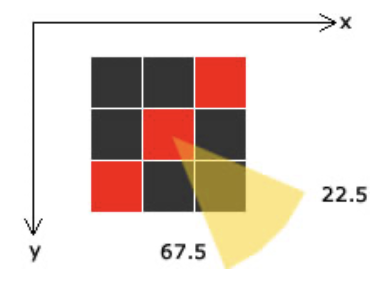
\includegraphics[scale=0.55]{figures/simple_NMS.png}
	\caption{简化版本的双线性插值}
\end{figure}

一个 NMS 的简化版本是把双线性插值省去,直接让这个像素的梯度大于它梯度方向的那两个相邻像素的梯度.

\subsection{Hysteresis Thresholding}

使用高阈值 (maxVal) 开始边缘曲线,使用低阈值 (minVal) 继续它们.

\begin{itemize}
    \item Pixels with gradient magnitudes > maxVal should be reserved.
    \item Pixels with gradient magnitudes < minVal should be removed.
\end{itemize}

How to decide maxVal and minVal? Examples:

\begin{itemize}
    \item maxVal = 0.3 $\times$ average magnitude of the pixels that pass NMS
    \item minVal = 0.1 $\times$ average magnitude of the pixels that pass NMS
\end{itemize}



\end{document}